% Figure from MATH 556 notes, section 40 (Lemma: nowhere dense via balls). From the board sketch (Lecture 15).
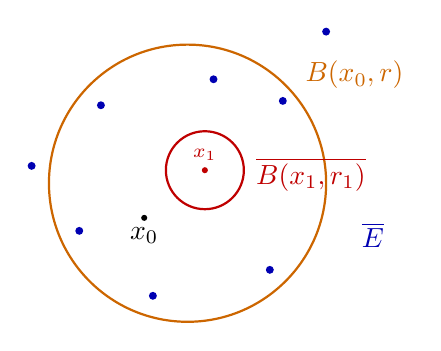
\begin{tikzpicture}[scale=1.1, >=stealth]
    \draw[thick, orange!80!black] (0,0) circle (1.6);
    \node[orange!80!black, anchor=west] at (1.25,1.25) {$B(x_0, r)$};
    \fill (-0.5,-0.4) circle (1pt) node[below] {$x_0$};
    \foreach \p in {(-1.0,0.9),(0.95,-1.0),(-1.25,-0.55),(1.1,0.95),(0.3,1.2),(-0.4,-1.3),(1.6,1.75),(-1.8,0.2)} {\fill[blue!70!black] \p circle (1.3pt);}
    \node[blue!70!black, anchor=west] at (1.9,-0.6) {$\overline{E}$};
    \draw[thick, red!75!black] (0.2,0.15) circle (0.45);
    \fill[red!75!black] (0.2,0.15) circle (1pt) node[above, font=\scriptsize] {$x_1$};
    \node[red!75!black, anchor=west] at (0.68,0.1) {$\overline{B(x_1, r_1)}$};
\end{tikzpicture}
